\documentclass[table]{article}
\usepackage[rgb,dvipsnames]{xcolor}
\usepackage{tikz}
\usepackage{iclr2017_conference,times}
\usepackage{amsmath, amsthm}
\usepackage[subscriptcorrection,mtpcal,amsbb]{mtpro2}
\usepackage{hyperref}
\usepackage{url}
\usepackage{enumitem}
\setlist{leftmargin=15pt}
\usepackage{inconsolata}
\usepackage{textcomp}
\usepackage{lastpage}
\cfoot{\thepage\ of \pageref{LastPage}}
\usepackage{makecell}
\usepackage{physics}
\usetikzlibrary{arrows,positioning,automata}
\usetikzlibrary{shapes.geometric}
\usepackage{float}
\usepackage{subcaption}
\usepackage{array}
\newcolumntype{L}[1]{>{\raggedright\let\newline\\\arraybackslash\hspace{0pt}}m{#1}}
\newcolumntype{C}[1]{>{\centering\let\newline\\\arraybackslash\hspace{0pt}}m{#1}}
\newcolumntype{R}[1]{>{\raggedleft\let\newline\\\arraybackslash\hspace{0pt}}m{#1}}
\usepackage{colortbl}
\usepackage{hhline}

\newcommand{\thickhline}{%
    \noalign {\ifnum 0=`}\fi \hrule height 1pt
    \futurelet \reserved@a \@xhline
}

\lhead{\textsc{IFT6135 Representation Learning}}
\rhead{S. Laferri\`ere \& J. Litalien}

\title{Assignment 2 --- Practical Part \\
Convolutional Neural Networks}

\author{Samuel Laferri\`ere\thanks{Student ID P0988904}\ \, \& Joey Litalien\thanks{Student ID P1195712} \\
IFT6135 Representation Learning, Winter 2018\\
Universit\'e de Montr\'eal\\
Prof. Aaron Courville \\
\texttt{$\{$samuel.laferriere.cyr,joey.litalien$\}$@umontreal.ca}}

\def\*#1{\mathbf{#1}}
\DeclareMathOperator{\ex}{\mathbb{E}}
\DeclareMathOperator{\Var}{Var}

\begin{document}
\maketitle
\thispagestyle{empty}

\section{Regularization}
\begin{enumerate}[label=(\alph*)]
\item \textit{Early stopping and weight decay.} We plot the $L^2$-norm of all parameters $\*w$ at each minibatch update for 100 epochs. To adapt the loss for minibatch SGD, we rescaled the regularization coefficient as $\lambda \gets \lambda b / |\*X|$, where $b$ is the batch size and $\*X$ is the entire training set. We also plot the average loss on the training set for both schemes.
\begin{figure}[ht]
\centering
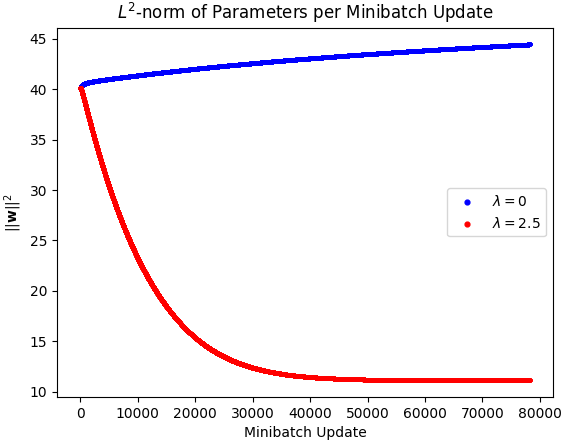
\includegraphics[scale=0.42]{1a_norm.png}
\vspace{5mm}

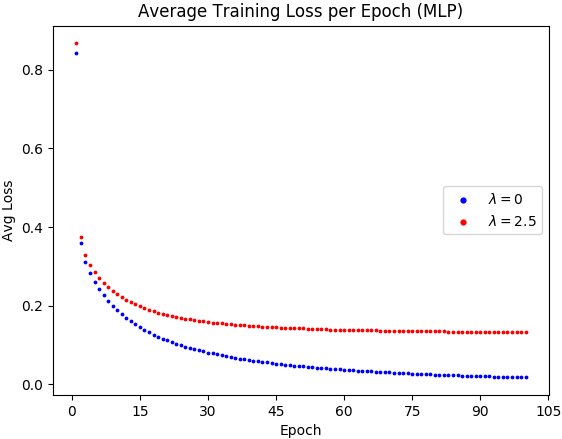
\includegraphics[scale=0.42]{1a_loss.png}
\end{figure}

 
 \newpage
\item \textit{Dropout.} We plot the accuracy for all three dropout schemes. We linked the data points for a better visualization. Note the straight line for the first scheme, as expected.

\begin{figure}[ht]
\centering
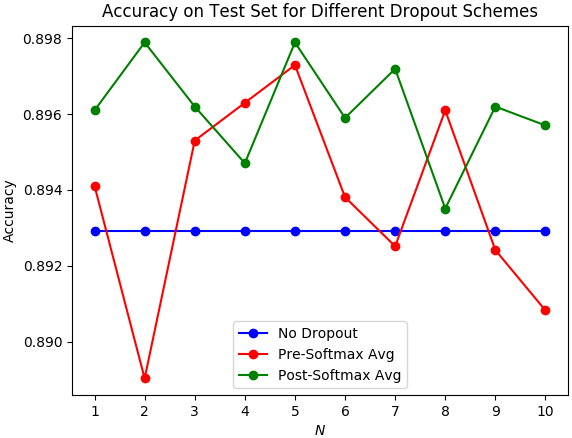
\includegraphics[scale=0.42]{1b_acc.png}
\end{figure}

\item \textit{Convolutional networks.}
We plot the error at the end of each epoch for the model.
\begin{figure}[ht]
\centering
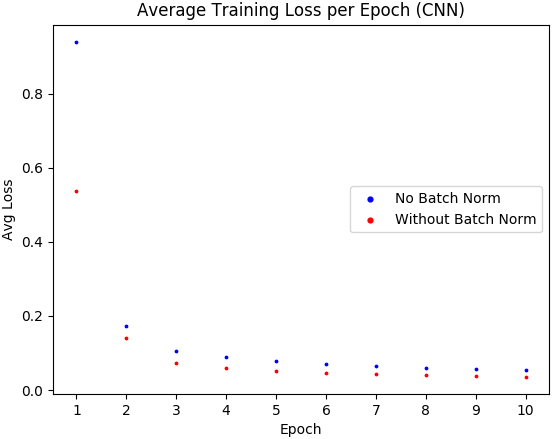
\includegraphics[scale=0.42]{1c_loss.png}
\end{figure}

\end{enumerate}

\newpage
\section{Dogs vs. Cats Classification}
We have resized the images to $3 \times 64 \times 64$ pixels using the Python script provided and separated the dataset into training/valid/test sets as follows. The index ranges apply to both dogs and cats, making each subsets' class distributions equal.
\begin{table}[ht]
\centering
\begin{tabular}{r C{6.3cm}  C{2.1cm} C{2.1cm} }�
Index range & \footnotesize{$[0, 7\,499$]} & \footnotesize{$[7\,500, 9\,999]$} & \footnotesize{$[10\,000,12\,499]$} \\ \hhline{~|*3-}
Dataset & \multicolumn{1}{|c}{\cellcolor{Blue!30}\textsc{Train}} & \multicolumn{1}{|c|}{\cellcolor{Red!30}\textsc{Valid}} & \multicolumn{1}{c|}
{\cellcolor{Yellow!30}\textsc{Test}} \\
\cline{2-4} 
Size & \footnotesize{15\,000} & \footnotesize{5\,000} & \footnotesize{5\,000} \\
\end{tabular}
\caption{Splitting the Dogs vs. Cats dataset.}
\end{table}

For all our experiments, we used a learning rate of 0.001 with standard momentum 0.9 and a batch size of 128. Moreover, we used ReLU activations for the last fully connected layer. We used Adam as the optimizer as it seemed to give better results than SGD in general, and trained using binary cross entropy.

\begin{enumerate}[label=(\alph*)]
\item \textit{Architecture.} We tried different features for the same architecture inspired from VGG. Our model is described below.
\begin{table}[ht]
\centering
\begin{tabular}{|c C{2.1cm} c|}
\multicolumn{3}{c}{\textbf{Vanilla}}\\
\multicolumn{3}{c}{}\\
\hline
\rowcolor{Blue!30}16 &Conv& $3 \times 3$ \\
\rowcolor{Blue!30}16 &Conv& $3 \times 3$ \\
\hline
\rowcolor{Red!30}&MaxPool &$2 \times 2$ \\
\hline
\hline
\rowcolor{Blue!30}32 &Conv& $3 \times 3$ \\
\rowcolor{Blue!30}32 &Conv& $3 \times 3$ \\
\hline
\rowcolor{Red!30}&MaxPool &$2 \times 2$ \\
\hline
\hline
\rowcolor{Blue!30}64 &Conv& $3 \times 3$ \\
\rowcolor{Blue!30}64 &Conv& $3 \times 3$ \\
\rowcolor{Blue!30}64 &Conv& $3 \times 3$ \\
\hline
\rowcolor{Red!30}&MaxPool &$2 \times 2$ \\
\hline
\hline
\rowcolor{Blue!30}128 &Conv& $3 \times 3$ \\
\rowcolor{Blue!30}128 &Conv& $3 \times 3$ \\
\rowcolor{Blue!30}128 &Conv& $3 \times 3$ \\
\hline
\rowcolor{Red!30}&MaxPool &$3 \times 3$ \\
\hline
\hline
\rowcolor{Yellow!30}2048 & Linear & 512  \\
\rowcolor{Yellow!30} & ReLU&  \\
\rowcolor{Yellow!30}512 & Linear & 2 \\
\hline
\multicolumn{3}{c}{}\\
\multicolumn{3}{c}{}\\
\multicolumn{3}{c}{}\\
\multicolumn{3}{c}{}\\
\multicolumn{3}{c}{}\\
\end{tabular}
\quad
\begin{tabular}{|c C{2.1cm} c|}
\multicolumn{3}{c}{\textbf{Augmented}}\\
\multicolumn{3}{c}{}\\
\hline
\rowcolor{Blue!30}16 &Conv& $3 \times 3$ \\
\rowcolor{Blue!30}16 &Conv& $3 \times 3$ \\
\hline
\rowcolor{Green!30}\multicolumn{3}{|c|}{BatchNorm / WeightNorm}\\
\hline
\rowcolor{Red!30}&MaxPool &$2 \times 2$ \\
\hline
\hline
\rowcolor{Blue!30}32 &Conv& $3 \times 3$ \\
\rowcolor{Blue!30}32 &Conv& $3 \times 3$ \\
\hline
\rowcolor{Green!30}\multicolumn{3}{|c|}{BatchNorm / WeightNorm}\\
\hline
\rowcolor{Red!30}&MaxPool &$2 \times 2$ \\
\hline
\hline
\rowcolor{Blue!30}64 &Conv& $3 \times 3$ \\
\rowcolor{Blue!30}64 &Conv& $3 \times 3$ \\
\rowcolor{Blue!30}64 &Conv& $3 \times 3$ \\
\hline
\rowcolor{Green!30}\multicolumn{3}{|c|}{BatchNorm / WeightNorm}\\
\hline
\rowcolor{Red!30}&MaxPool &$2 \times 2$ \\
\hline
\hline
\rowcolor{Blue!30}128 &Conv& $3 \times 3$ \\
\rowcolor{Blue!30}128 &Conv& $3 \times 3$ \\
\rowcolor{Blue!30}128 &Conv& $3 \times 3$ \\
\hline
\rowcolor{Green!30}\multicolumn{3}{|c|}{BatchNorm / WeightNorm}\\
\hline
\rowcolor{Red!30}&MaxPool2D &$3 \times 3$ \\
\hline
\hline
\rowcolor{Yellow!30}2048 & Linear & 512  \\
\rowcolor{Yellow!30} & ReLU  & \\
\rowcolor{Yellow!30} &Dropout&0.5\\
\rowcolor{Yellow!30}512 & Linear & 2 \\
\hline
\end{tabular}
\caption{Model architecture for Dogs vs. Cats.}
\end{table}


\item \textit{Performance on test set.}
\item \textit{Visualization and possible improvements.}
\end{enumerate}

















\end{document}